%%%%%%%%%%%%%%
%% Run LaTeX on this file several times to get Table of Contents,
%% cross-references, and citations.

%% If you have font problems, you may edit the w-bookps.sty file
%% to customize the font names to match those on your system.

%% w-bksamp.tex. Current Version: Feb 16, 2012
%%%%%%%%%%%%%%%%%%%%%%%%%%%%%%%%%%%%%%%%%%%%%%%%%%%%%%%%%%%%%%%%
%
%  Sample file for
%  Wiley Book Style, Design No.: SD 001B, 7x10
%  Wiley Book Style, Design No.: SD 004B, 6x9
%
%
%  Prepared by Amy Hendrickson, TeXnology Inc.
%  http://www.texnology.com
%%%%%%%%%%%%%%%%%%%%%%%%%%%%%%%%%%%%%%%%%%%%%%%%%%%%%%%%%%%%%%%%

%%%%%%%%%%%%%
% 7x10
%\documentclass{wileySev}

% 6x9
\documentclass{wileySix}

\usepackage{graphicx}
\usepackage{listings}
\usepackage{float}
\usepackage[urlcolor=blue, colorlinks=true]{hyperref}
\usepackage{textcomp}
\usepackage{color}
 
\definecolor{codegreen}{rgb}{0,0.6,0}
\definecolor{codegray}{rgb}{0.5,0.5,0.5}
\definecolor{codepurple}{rgb}{0.58,0,0.82}
\definecolor{backcolour}{rgb}{0.95,0.95,0.92}
 
\lstdefinestyle{mystyle}{
    backgroundcolor=\color{backcolour},   
    commentstyle=\color{codegreen},
    keywordstyle=\color{magenta},
    numberstyle=\tiny\color{codegray},
    stringstyle=\color{codepurple},
    basicstyle=\footnotesize,
    breakatwhitespace=false,         
    breaklines=true,                 
    captionpos=b,                    
    keepspaces=true,                 
    numbers=left,                    
    numbersep=5pt,                  
    showspaces=false,                
    showstringspaces=false,
    showtabs=false,                  
    tabsize=2,
    language=sh
}
 
\lstset{style=mystyle}

%%%%%%%
%% for times math: However, this package disables bold math (!)
%% \mathbf{x} will still work, but you will not have bold math
%% in section heads or chapter titles. If you don't use math
%% in those environments, mathptmx might be a good choice.

% \usepackage{mathptmx}

% For PostScript text
%\usepackage{w-bookps}

%%%%%%%%%%%%%%%%%%%%%%%%%%%%%%%%%%%%%%%%%%%%%%%%%%%%%%%%%%%%%%%%
%% Other packages you might want to use:

% for chapter bibliography made with BibTeX
% \usepackage{chapterbib}

% for multiple indices
% \usepackage{multind}

% for answers to problems
% \usepackage{answers}

%%%%%%%%%%%%%%%%%%%%%%%%%%%%%%
%% Change options here if you want:
%%
%% How many levels of section head would you like numbered?
%% 0= no section numbers, 1= section, 2= subsection, 3= subsubsection
%%==>>
\setcounter{secnumdepth}{3}

%% How many levels of section head would you like to appear in the
%% Table of Contents?
%% 0= chapter titles, 1= section titles, 2= subsection titles, 
%% 3= subsubsection titles.
%%==>>
\setcounter{tocdepth}{2}

%% Cropmarks? good for final page makeup
%% \docropmarks

%%%%%%%%%%%%%%%%%%%%%%%%%%%%%%
%
% DRAFT
%
% Uncomment to get double spacing between lines, current date and time
% printed at bottom of page.
% \draft
% (If you want to keep tables from becoming double spaced also uncomment
% this):
% \renewcommand{\arraystretch}{0.6}
%%%%%%%%%%%%%%%%%%%%%%%%%%%%%%

%%%%%%% Demo of section head containing sample macro:
%% To get a macro to expand correctly in a section head, with upper and
%% lower case math, put the definition and set the box 
%% before \begin{document}, so that when it appears in the 
%% table of contents it will also work:

\newcommand{\VT}[1]{\ensuremath{{V_{T#1}}}}

%% use a box to expand the macro before we put it into the section head:

\newbox\sectsavebox
\setbox\sectsavebox=\hbox{\boldmath\VT{xyz}}

%%%%%%%%%%%%%%%%% End Demo


\begin{document}


\booktitle{Cerdas Menguasai Git}
\subtitle{Dalam 24 Jam}

\authors{Rolly M. Awangga\\
\affil{Informatics Research Center}
%Floyd J. Fowler, Jr.\\
%\affil{University of New Mexico}
}

\offprintinfo{Cerdas Menguasai Git, First Edition}{Rolly M. Awangga}

%% Can use \\ if title, and edition are too wide, ie,
%% \offprintinfo{Survey Methodology,\\ Second Edition}{Robert M. Groves}

%%%%%%%%%%%%%%%%%%%%%%%%%%%%%%
%% 
\halftitlepage

\titlepage


\begin{copyrightpage}{2019}
\input{info/copyrightpage}
\end{copyrightpage}

\dedication{`Jika Kamu tidak dapat menahan lelahnya belajar, 
Maka kamu harus sanggup menahan perihnya Kebodohan.'
~Imam Syafi'i~}

\begin{contributors}
\input{info/contributors}
\end{contributors}

\contentsinbrief
\tableofcontents
\listoffigures
\listoftables
\lstlistoflistings


\begin{foreword}
\input{info/foreword}
\end{foreword}

\begin{preface}
\input{info/preface}
\end{preface}


\begin{acknowledgments}
\input{info/acknowledgments}
\end{acknowledgments}

\begin{acronyms}
\input{info/acronyms}
\end{acronyms}

\begin{glossary}
\input{info/glossary}
\end{glossary}

\begin{symbols}
\input{info/symbols}
\end{symbols}

\begin{introduction}
\input{info/introduction}
\end{introduction}

%%%%%%%%%%%%%%%%%%Isi Buku_

\chapter{Chapter 1}
\input{chapters/chapter1/1174006}
\section{1174035 Luthfi Muhammad Nabil}
Kecerdasan buatan merupakan kecerdasan yang dimasukkan ke sistem yang dapat diatur untuk kepentingan ilmiah. Kecerdasan buatan biasa disebut AI (Artificial Intelligence) yang didefinisikan sebagai kecerdasan ilmiah. AI memiliki kemampuan untuk menerjemahkan data dari luar, dan mempelajari data tersebut untuk dipelajari demi mencapai tujuan dan melakukan tugas tertentu sesuai hasil adaptasi berdasarkan data yang didapat. 

\subsection{Sejarah dan perkembangaan Kecerdasan Buatan}
AI mulai berkembang sesuai dengan konsep yang dikemukakan pada awal abad 17, Rene Descartes menyebutkan bahwa tubuh hewan bukanlah apa-apa melainkan mesin-mesin yang rumit. Lalu Blaise Pascal menciptakan mesin perhitungan digital mekanis pertama pada 1642. Selanjutnya pada abad ke 19, Charles Babbage dan Ada Lovelace menciptakan sebuah mesin penghitung mekanis yang dapat diprogram.

Pada tahun 1950-an, Program AI pertama yang sudah dapat difungsikan telah ditulis pada 1951 untuk menjalankan mesin Ferranti Mark I di University of Manchester yang merupakan sebuah program permainan naskah yang ditulis oleh Christopher Strachey. John McCarthy menyebutkan istilah "kecerdasan buatan" pada konferensi pertama yang disediakan untuk persoalan ini. Dilanjut pada tahun 1956, Beliau menemukan bahasa pemrograman yang bernama Lisp.

Jaringan saraf mulai digunakan secara luas pada tahun 1980-an, dimana algoritma perambatan balik pertama kali dijelaskan oleh Paul John Werbos pada tahun 1974. Selanjutnya di tahun 1982, para ahli fisika menganalisis sifat dari penyimpanan dan optimasi pada jaringan saraf menggunakan sistem statistika. Lalu dilanjutkan pada tahun 1985 sedikitnya empat kelompok riset menemukan algoritma pembelajaran propagansi balik. Algoritma ini berhasil diimplementasikan ke ilmu komputer dan psikologi. Dan pada tahun 1990, ditandai perolehan besar dalam berbagai bidang AI dan demonstrasi dari berbagai aplikasi yang sudah mengimplementasi. Seperti Deep Blue, sebuah komputer dari permainan catur yang dapat mengalahkan Garry Kasparov dalam sebuah pertandingan 6 game yang terkenal pada 1997. 

\subsection{Supervised Learning}
Supervised learning adalah kondisi yang menggunakan variabel input dan output untuk dapat dilakukan pemetaan input output yang sudah didapat. Disebud Supervised Learning karena proses dari pembelajaran algoritma dari pembelajan yang disumberkan dengan dataset dapat dipikirkan seperti seorang guru yang mengawasi proses pembelajaran. Proses pembelajaran dari algoritma akan berhenti saat algoritma sudah mendapatkan level dari performansi yang dapat diteriima.
\hfill\break
Masalah dari Supervised learning dapat dikelompokkan menjadi masalah dengan regresi dan klasifikasi
\begin{itemize}
	\item Klasifikasi : Masalah dalam klasifikasi yang dimana output dari variable itu adalah kategori, seperti "Laki - laki" atau "Perempuan, dan "Muda" dan "Tua"
	\item Regresi : Masalah dalam regresi adalah jika pengeluaran dari variabel adalah sebuah nilai asli, seperti "suhu", dan "tinggi"
\end{itemize}

\subsection{Unsupervised Learning}
Unsupervised learning adalah kondisi dimana kamu hanya memiliki input data tanpa memiliki variabel output yang sesuai. Tujuan dari unsupervised learning adalah untuk memodelkan distribusi pada data untuk mengetahui lebih lanjut mengenai data. Disebut unsupervised learning karena pada metode ini, tidak ada jawaban yang tepat dan tidak ada pengarah. Sehingga algoritma akan ditinggalkan sesuai rancangan demi menemukan dan dapat mengolah data yang menarik pada saat yang akan datang. 

\subsection{Jenis - Jenis Dataset}
Dataset merupakan objek yang merepresentasikan data dan relasinya di memor. Strukturnya dapat mirip sesuai dengan struktur yang ada pada database namun bisa diubah sesuai dengan kebutuhan. Dataset juga berisi koleksi dari tabel data dan relasi data.
\begin{itemize}
	\item Training set : merupakan sebuah dataset yang digunakan untuk kepentingan pembelajaran. Kepentingan tersebut akan disesuaikan dengan parameter yang ada. 
	\item Test dataset : adalah sebuah dataset yang bersifat independen dibandingkan dengan training dataset, namun mengikuti probabilitas distribusi yang sama dengan training dataset. Jika model sudah sesuai dengan training dataset maka dataset sudah dapat disesuaikan dengan test dataset. Penyesuaian dari training dataset .
\end{itemize}

\subsection{Instalasi dan Percobaan Kompilasi dari Library Scikit-learn}
\begin{enumerate}
	\item Buka anaconda prompt
	\item Ketik di anaconda prompt yaitu : "pip install -U scikit-learn" untuk instalasi \hfill \break
	\begin{figure}[H]
		\includegraphics[width=4cm]{figures/1174035/chapter1/1_1.png}
		\centering
		\caption{Instalasi Scikit Learn}
	\end{figure}
	\item Setelah selesai instalasi, pilih salah satu example dari website Scikit (Contoh : \href{https://scikit-learn.org/stable/auto_examples/index.html})
	\begin{figure}[H]
		\includegraphics[width=4cm]{figures/1174035/chapter1/1_2.png}
		\centering
		\caption{Daftar Example}
	\end{figure}
	\item Lalu coba jalankan aplikasi tersebut, bisa dicek hasil dari Variable explorernya
	\begin{figure}[H]
		\includegraphics[width=4cm]{figures/1174035/chapter1/1_3.png}
		\centering
		\caption{Variable Explorer}
	\end{figure}
	\item Sample kode \hfill \break \lstinputlisting[firstline=1]{src/1174035/chapter1/sample1.py}
\end{enumerate}

\subsection{Mencoba Loading and example dataset}
Disini akan dilakukan percobaan dengan menggunakan beberapa datasets seperti digits dan iris untuk bisa digunakan sebagai training set yang akan dipakai seluruh metode.
\begin{itemize}
	\item Percobaan 1 (Memuat data iris dan digits dari datasets) \hfill \break \lstinputlisting[firstline=8, lastline=10]{src/1174035/chapter1/sample2.py}
	\begin{figure}[H]
		\includegraphics[width=4cm]{figures/1174035/chapter1/2_1_hasil.png}
		\centering
		\caption{Hasil Percobaan 1}
		
	\end{figure}
	\item Percobaan 2 (Menampilkan data dari digits) \hfill \break \lstinputlisting[firstline=12, lastline=12]{src/1174035/chapter1/sample2.py}
	\begin{figure}[H]S
		\includegraphics[width=4cm]{figures/1174035/chapter1/2_2_hasil.png}
		\centering
		\caption{Hasil Percobaan 2}
	\end{figure}
	\item Percobaan 3 (Menampilkan digits.target) \hfill \break \lstinputlisting[firstline=14, lastline=14]{src/1174035/chapter1/sample2.py}
	\begin{figure}[H]
		\includegraphics[width=4cm]{figures/1174035/chapter1/2_3_hasil.png}
		\centering
		\caption{Hasil Percobaan 3}
	\end{figure}
	\item Percobaan 4 (Menampilkan data 2 dimensi) \hfill \break \lstinputlisting[firstline=16, lastline=16]{src/1174035/chapter1/sample2.py}
	\begin{figure}[H]
		\includegraphics[width=4cm]{figures/1174035/chapter1/2_4_hasil.png}
		\centering
		\caption{Hasil Percobaan 4}
	\end{figure}
	\item Full sample \hfill \break \lstinputlisting[firstline=1]{src/1174035/chapter1/sample2.py}
	\begin{figure}[H]
		\includegraphics[width=4cm]{figures/1174035/chapter1/2_var.png}
		\centering
		\caption{Hasil pada variable explorer}
	\end{figure}
\end{itemize}
\subsection{Learning and Predicting}
Disini akan dicoba untuk melakukan prediksi berupa angka yang inputnya berupa gambaran dataset. 
\begin{itemize}
	\item Percobaan 1  \hfill \break \lstinputlisting[firstline=8, lastline=11]{src/1174035/chapter1/sample3.py}
	\begin{figure}[H]
		\includegraphics[width=4cm]{figures/1174035/chapter1/3_1_hasil.png}
		\centering
		\caption{Hasil Percobaan 1}
	\end{figure}
	\item Percobaan 2 \hfill \break \lstinputlisting[firstline=13, lastline=14]{src/1174035/chapter1/sample3.py}
	\begin{figure}[H]
		\includegraphics[width=4cm]{figures/1174035/chapter1/3_2_hasil.png}
		\centering
		\caption{Hasil Percobaan 2}
	\end{figure}
	\item Percobaan 3  \hfill \break \lstinputlisting[firstline=16, lastline=16]{src/1174035/chapter1/sample3.py}
	\begin{figure}[H]
		\includegraphics[width=4cm]{figures/1174035/chapter1/3_3_hasil.png}
		\centering
		\caption{Hasil Percobaan 3}
	\end{figure}
	\item Full sample \hfill \break \lstinputlisting[firstline=1]{src/1174035/chapter1/sample3.py}
	\begin{figure}[H]
		\includegraphics[width=4cm]{figures/1174035/chapter1/3_var.png}
		\centering
		\caption{Hasil pada variable explorer}
	\end{figure}
\end{itemize}
\subsection{Model Persistence}
Disini akan dilakukan persistensi model menggunakan built-in dari Python
\begin{itemize}
	\item Percobaan 1  \hfill \break \lstinputlisting[firstline=8, lastline=12]{src/1174035/chapter1/sample4.py}
	\begin{figure}[H]
		\includegraphics[width=4cm]{figures/1174035/chapter1/4_1_hasil.png}
		\centering
		\caption{Hasil Percobaan 1}
	\end{figure}
	\item Percobaan 2 \hfill \break \lstinputlisting[firstline=14, lastline=17]{src/1174035/chapter1/sample4.py}
	\begin{figure}[H]
		\includegraphics[width=4cm]{figures/1174035/chapter1/4_2_hasil.png}
		\centering
		\caption{Hasil Percobaan 2}
	\end{figure}
	\item Percobaan 3  \hfill \break \lstinputlisting[firstline=19, lastline=19]{src/1174035/chapter1/sample4.py}
	\begin{figure}[H]
		\includegraphics[width=4cm]{figures/1174035/chapter1/4_3_hasil.png}
		\centering
		\caption{Hasil Percobaan 3}
	\end{figure}
	\item Percobaan 4  \hfill \break \lstinputlisting[firstline=21, lastline=22]{src/1174035/chapter1/sample4.py}
	\begin{figure}[H]
		\includegraphics[width=4cm]{figures/1174035/chapter1/4_4_hasil.png}
		\centering
		\caption{Hasil Percobaan 4}
	\end{figure}
	\item Percobaan 5  \hfill \break \lstinputlisting[firstline=24, lastline=24]{src/1174035/chapter1/sample4.py}
	\begin{figure}[H]
		\includegraphics[width=4cm]{figures/1174035/chapter1/4_5_hasil.png}
		\centering
		\caption{Hasil Percobaan 5}
	\end{figure}
	\item Full sample \hfill \break \lstinputlisting[firstline=1]{src/1174035/chapter1/sample4.py}
	\begin{figure}[H]
		\includegraphics[width=4cm]{figures/1174035/chapter1/4_var.png}
		\centering
		\caption{Hasil pada variable explorer}
	\end{figure}
\end{itemize}
\subsection{Conventions}
Seluruh metode akan dilakukan pengaturan untuk membuat tingkah laku lebih dapat diprediksi
\begin{itemize}
	\item Percobaan 1  \hfill \break \lstinputlisting[firstline=8, lastline=14]{src/1174035/chapter1/sample5.py}
	\begin{figure}[H]
		\includegraphics[width=4cm]{figures/1174035/chapter1/5_1_hasil.png}
		\centering
		\caption{Hasil Percobaan 1}
	\end{figure}
	\item Percobaan 2 \hfill \break \lstinputlisting[firstline=16, lastline=18]{src/1174035/chapter1/sample5.py}
	\begin{figure}[H]
		\includegraphics[width=4cm]{figures/1174035/chapter1/5_2_hasil.png}
		\centering
		\caption{Hasil Percobaan 2}
	\end{figure}
	\item Percobaan 3  \hfill \break \lstinputlisting[firstline=21, lastline=25]{src/1174035/chapter1/sample5.py}
	\begin{figure}[H]
		\includegraphics[width=4cm]{figures/1174035/chapter1/5_3_hasil.png}
		\centering
		\caption{Hasil Percobaan 3}
	\end{figure}
	\item Percobaan 4  \hfill \break \lstinputlisting[firstline=27, lastline=27]{src/1174035/chapter1/sample5.py}
	\begin{figure}[H]
		\includegraphics[width=4cm]{figures/1174035/chapter1/5_4_hasil.png}
		\centering
		\caption{Hasil Percobaan 4}
	\end{figure}
	\item Percobaan 5  \hfill \break \lstinputlisting[firstline=29, lastline=29]{src/1174035/chapter1/sample5.py}
	\begin{figure}[H]
		\includegraphics[width=4cm]{figures/1174035/chapter1/5_5_hasil.png}
		\centering
		\caption{Hasil Percobaan 5}
	\end{figure}
	\item Percobaan 6  \hfill \break \lstinputlisting[firstline=31, lastline=31]{src/1174035/chapter1/sample5.py}
	\begin{figure}[H]
		\includegraphics[width=4cm]{figures/1174035/chapter1/5_6_hasil.png}
		\centering
		\caption{Hasil Percobaan 6}
	\end{figure}
	\item Full sample \hfill \break \lstinputlisting[firstline=1]{src/1174035/chapter1/sample5.py}
	\begin{figure}[H]
		\includegraphics[width=4cm]{figures/1174035/chapter1/5_var.png}
		\centering
		\caption{Hasil pada variable explorer}
	\end{figure}
\end{itemize}
\subsection{Skrinsut Error}
\begin{figure}[H]
	\includegraphics[width=4cm]{figures/1174035/chapter1/skrinsuterror.png}
	\centering
	\caption{Hasil Percobaan 6}
\end{figure}
\subsection{Kode error dan jenis error tersebut}
Error yang didapat berjenis name error, karena sebuah variabel tidak didefinisikan. Yaitu digits
\lstinputlisting[firstline=1]{src/1174035/chapter1/sample5.py}
\subsection{Penanganan Error}
Untuk menangani error tersebut, bisa ditambahkan sesuai instruksi. Yaitu menambahkan sebuah variabel bernama digits. Selain itu, digits harus dapat bekerja sebagaimana mestinya. Berikut full kodingnya : 
\lstinputlisting[firstline=1]{src/1174035/chapter1/sample3.py}
\subsection{Plagiarisme}
\begin{figure}[H]
	\includegraphics[width=4cm]{figures/1174035/chapter1/plagiarism.png}
	\centering
	\caption{Hasil pada variable explorer}
\end{figure}
\input{chapters/chapter1/1174040}
\section{1174042 Faisal Najib Abdullah}

\subsection{Teori}
\begin{enumerate}

        \item Jelaskan dengan ilustrasi gambar sendiri apa perbedaan antara vanilla GAN dan cGAN.
		Generator dan Disciminator pada Vanilla GAN adalah pembelajaran multi-layer yang sederhana, dimana algoritmanya sederhana yang mencoba untuk mengoptimasi persamman matematika menggunakan penurunan gradien stokastik. Sedangkan cGAN dapat dideskripsikan sebagai deep learing pada parameter kondisional diberlakukan.
			\begin{figure}[H]
            	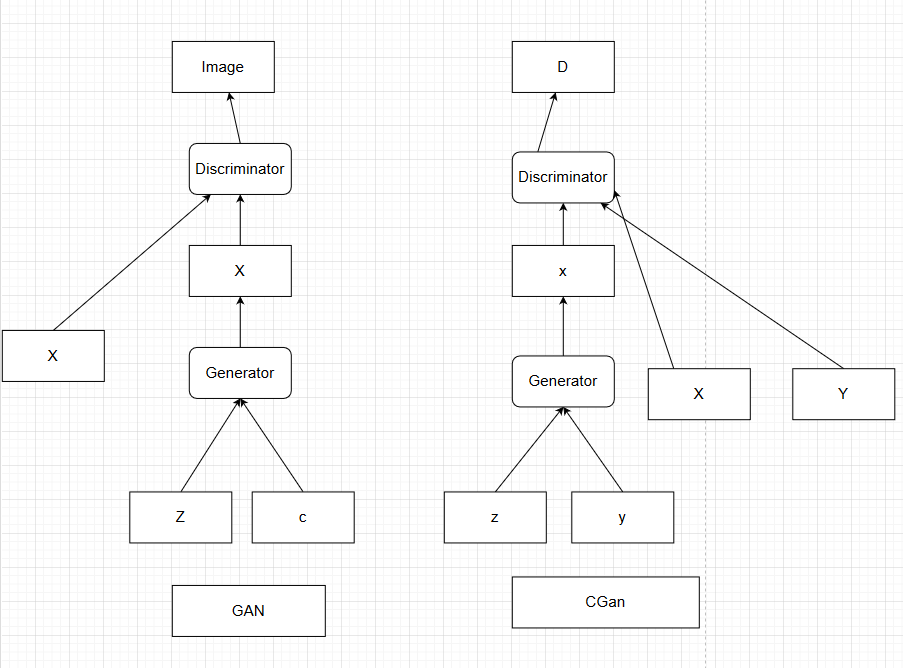
\includegraphics[width=4cm]{figures/1174042/chapter9/teori1.PNG}
           		\centering
           		\caption{Valina GAN-cGAN}
            \end{figure}
            
        \item Jelaskan dengan ilustrasi gambar sendiri arsitektur dari Age-cGAN.
		Age cGAN mempunyai 4 jaringan yang  di latih dalam 3 tahapan yaitu: Conditional GAN Training,Initial latent vector approximation,dan Latent vector optimization.
			\begin{figure}[H]
				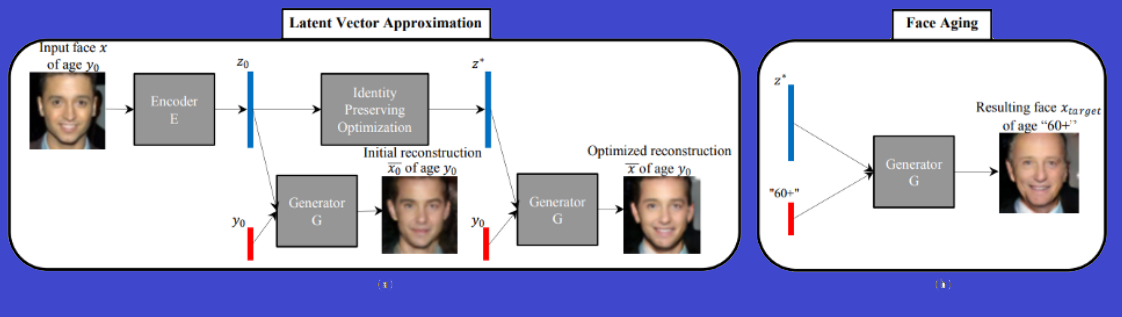
\includegraphics[width=4cm]{figures/1174042/chapter9/teori2.PNG}
            		\centering
           		\caption{Age-cGAN}
            \end{figure}
                
        \item Jelaskan dengan ilustrasi gambar sendiri arsitektur encoder network dari AgecGAN.
		Arsitektur encoder biasanya digunakan untuk mengenerate latent vector dari gambar yang akan diinputkan yang nantinya akan diteruskan ke generator.
            \begin{figure}[H]
                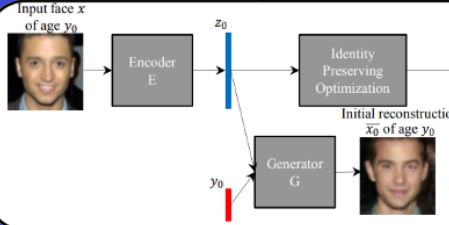
\includegraphics[width=4cm]{figures/1174042/chapter9/teori3.PNG}
                    \centering
                \caption{Encoder Age cGANr}
            \end{figure}

        \item Jelaskan dengan ilustrasi gambar sendiri arsitektur generator network dari AgecGAN.
		Arsitektur generator adalah sebuah CNN dan mengambil 100-dimensional latent vector sebagai inputannya yang akan menghasilkan gambar realistik dalam dimensi (64,64,3)
		\begin{figure}[H]
			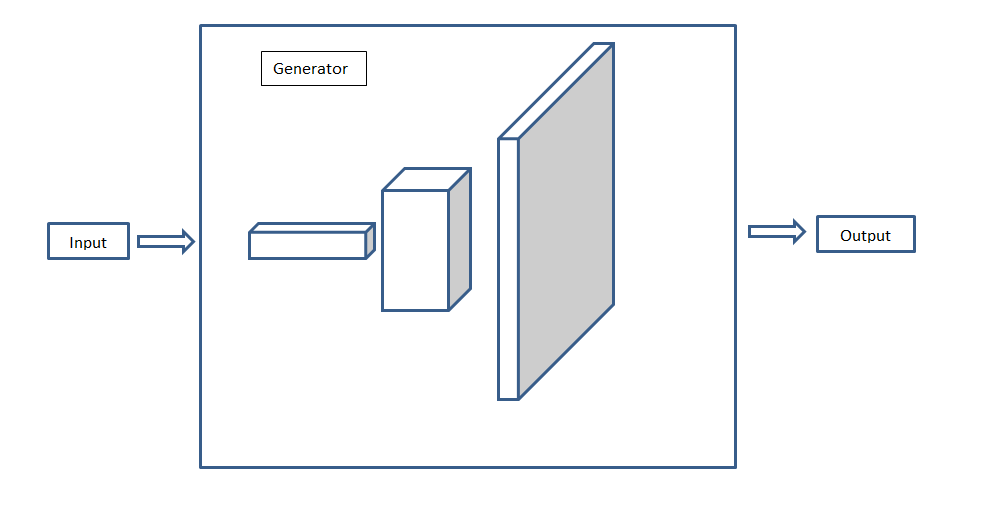
\includegraphics[width=4cm]{figures/1174042/chapter9/teori4.PNG}
            	\centering
           	\caption{Network Age cGAN}
       	\end{figure}


        \item Jelaskan dengan ilustrasi gambar sendiri arsitektur discriminator network dari Age-cGAN.
		Arsitektur diskriminator adalah CNN yang fungsinya untuk memprediksi apakah gambar yang diberikan palsu atau asli.
		\begin{figure}[H]
			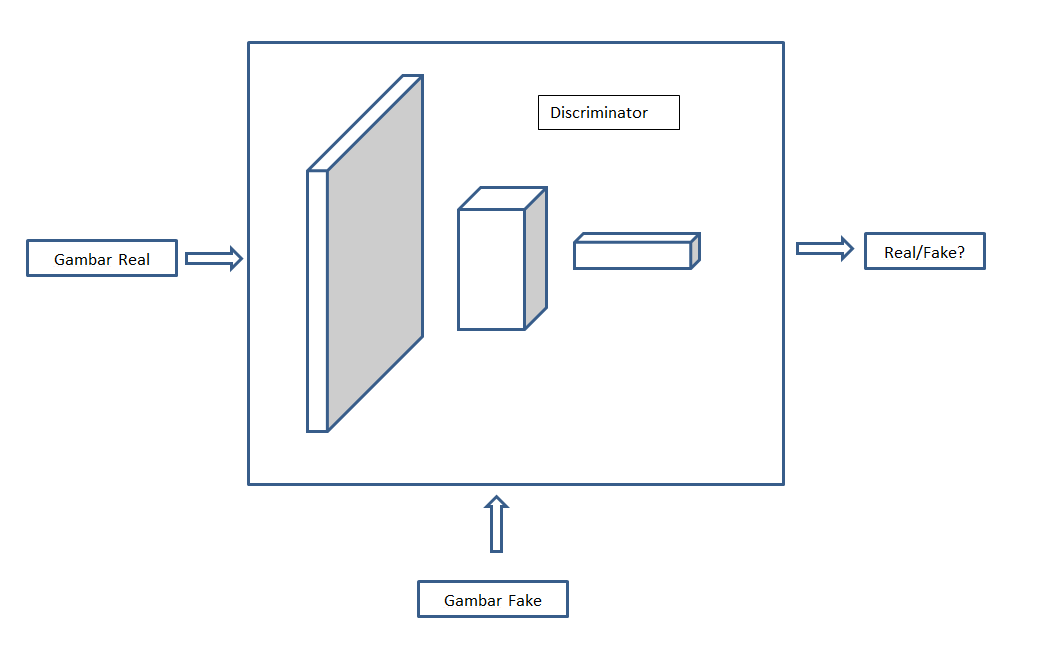
\includegraphics[width=4cm]{figures/1174042/chapter9/teori5.PNG}
            	\centering
           	\caption{Discriminator Age cGAN}
       	\end{figure}


        \item Jelaskan dengan ilustrasi gambar apa itu pre-trained Inception-ResNet-2 Model.
		Pre-Trained Network atau Transfer Learning merupakan suatu metode penyelesaian yang memanfaatkan model yang sudah dilatih terhadap suatu dataset untuk menyelesaikan masalah dengan cara menggunakan sebagai starting point, memodifikasi dan mengupdate parameternya, sehingga sesuai dengan dataset yang baru.
		\begin{figure}[H]
			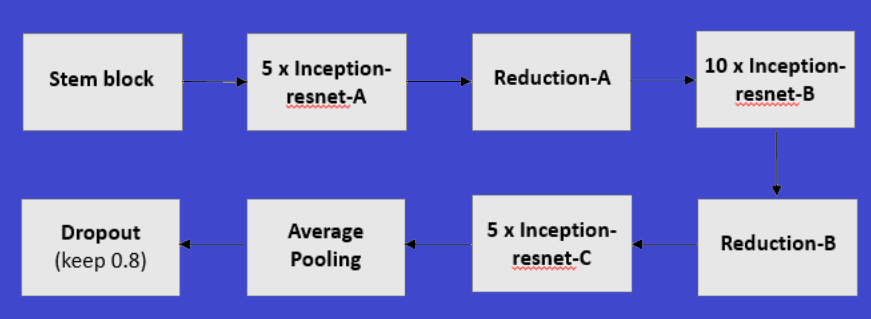
\includegraphics[width=4cm]{figures/1174042/chapter9/teori6.PNG}
            	\centering
           	\caption{Pretrained Inception ResNet}
       	\end{figure}

        \item Jelaskan dengan ilustrasi gambar sendiri arsitektur Face recognition network Age-cGAN.
		Face Recognition digunakan untuk mengenali identitas seseorang dari gambar yang diberikan.
		\begin{figure}[H]
			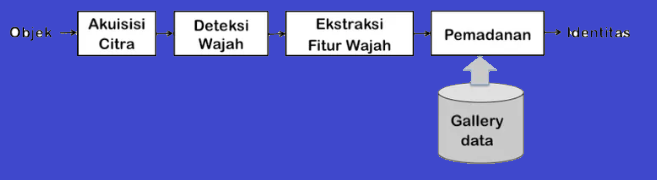
\includegraphics[width=4cm]{figures/1174042/chapter9/teori7.PNG}
            	\centering
           	 \caption{Face recognition network Age-cGAN}
       	 \end{figure}

        \item Sebutkan dan jelaskan serta di sertai contoh-contoh tahapan dari Age-cGAN.
		Pada dari Age-cGan ni terdapat 2 tahapan dengan generator dan diskriminator. dimana untuk tahap generator sendiri membutuhkan vektor laten 100 serta menghasilkan gambar yang realistis dari dimensinya. sedangkan tahap diskriminator itu tahapan dimana memprediksi gambar yang diberikan nyata atau palsu.
		\begin{figure}[H]
			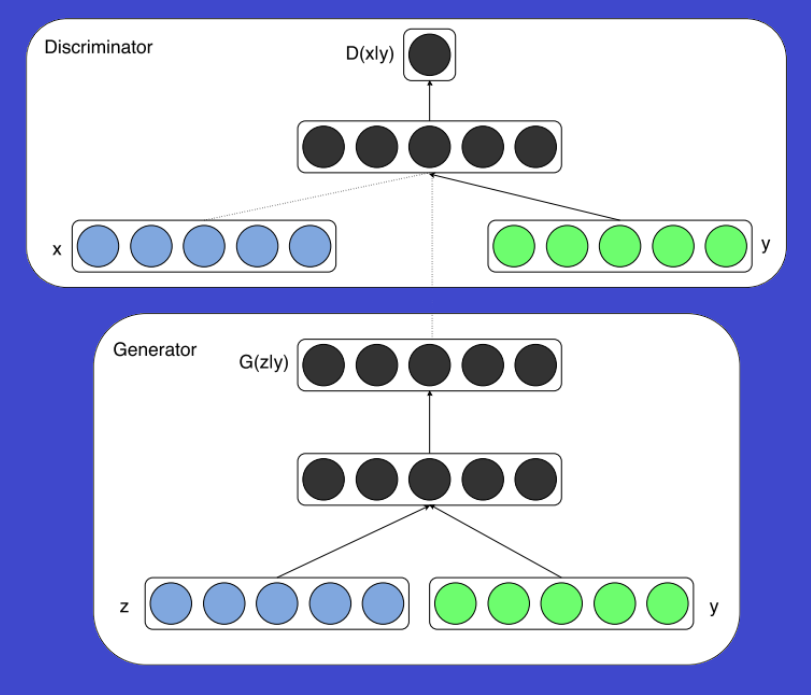
\includegraphics[width=4cm]{figures/1174042/chapter9/teori8.PNG}
            	\centering
           	 \caption{Tahap Age cGAN}
       	\end{figure}

        \item Berikan contoh perhitungan fungsi training objektif.
		Objektif Trainning ialah untuk meminimalkan loss function sebagai log likelihood function yang diberikan pada persamaan dimana D melambangkan trainning data.
		\begin{figure}[H]
			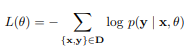
\includegraphics[width=4cm]{figures/1174042/chapter9/teori9.PNG}
            	\centering
           	 \caption{Training Objektif}
       	\end{figure}

        \item Berikan contoh dengan ilustrasi penjelasan dari Initial latent vector approximation.
		Latent vector approdimation kemampuan untuk membuat gamar yang realistis dan tajam serta menghasilkan gambar wajah pada usia target.
		\begin{figure}[H]
			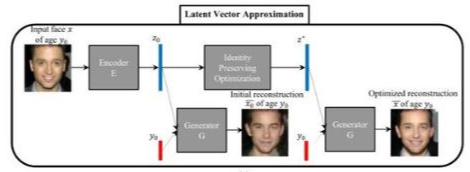
\includegraphics[width=4cm]{figures/1174042/chapter9/teori10.PNG}
            	\centering
           	 \caption{Initial Latent Vector Approximation}
       	\end{figure}

        \item Berikan contoh perhitungan latent vector optimization.
		Perhitungan lantent optimization menggunakan metode yang relatif sederhana, tergantung pada jumlah kecil parameter yang diperlukan, sehingga pada latent optimization dapat memetakan setiap gambar x dari dataset ke vektor acak dimensi rendah zi dalam ruang laten z.
		\begin{figure}[H]
			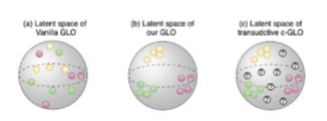
\includegraphics[width=4cm]{figures/1174042/chapter9/teori11.PNG}
            	\centering
           	\caption{Latent Vector Optimization}
        \end{figure}
           
\end{enumerate}

\subsection{Praktek}

    \begin{enumerate}
	\item Jelaskan bagaimana cara ekstrak file dataset Age-cGAN menggunakan google colab.
    Kode dibawah ini digunakan untuk membuat notebooks baru, kemudian membuat ekstraksi file dari link dataset.
	\lstinputlisting[firstline=1, lastline=4]{src/1174042/chapter9/1174042.py}

	\item Jelaskan bagaimana kode program bekerja untuk melakukan load terhadap dataset yang sudah di ekstrak, termasuk bagaimana penjelasan kode program perhitungan usia.
    Kode dibawah berfungsi untuk melakukan fungsi perhitungan usia.
	\lstinputlisting[firstline=6, lastline=31]{src/1174042/chapter9/1174042.py}

	\item Jelaskan bagaimana kode program The Encoder Network bekerja dijelaskan dengan bahawa awam dengan ilustrasi sederhana.
    Berikut adalah proses Encoder dengan vector latent Z yang berfungsi untuk mempelajari pemetaan terbalik dari gambar wajah dan kondisi usia .
	\lstinputlisting[firstline=33, lastline=73]{src/1174042/chapter9/1174042.py}

	\item Jelaskan bagaimana kode program The Generator Network bekerja dijelaskan dengan bahawa awam dengan ilustrasi sederhana.
    Proses Generator agar bekerja dengan baik dibutuhkan representasi dari gambar wajah dan vector kondisi sebagai inputan yang menghasilkan sebuah gambar.
	\lstinputlisting[firstline=75, lastline=104]{src/1174042/chapter9/1174042.py}

    \item Jelaskan bagaimana kode program The Discriminator Network bekerja dijelaskan dengan bahawa awam dengan ilustrasi sederhana.
    Berikut adalah proses Discriminator yang digunakan untuk membedakan antara gambar asli ataupun gambar palsu yang dihasilkan oleh generator.
	\lstinputlisting[firstline=116, lastline=148]{src/1174042/chapter9/1174042.py}

    \item Jelaskan bagaimana kode program Training cGAN bekerja dijelaskan dengan bahawa awam dengan ilustrasi sederhana.
    Proses Training cGAN ini dengan load file .mat pada dataset lalu epoch sebanuak 500 kali.

	\lstinputlisting[firstline=150, lastline=167]{src/1174042/chapter9/1174042.py}

    \item Jelaskan bagaimana kode program Initial dan latent vector approximation bekerja dijelaskan dengan bahawa awam dengan ilustrasi sederhana.
    Initial dan Latent Vector Approximation bekerja melakukan predicsi epoch yang telah di buat sebanyak 500 kali, dan nanti hasilnya ada di folder result.

	\lstinputlisting[firstline=169, lastline=217]{src/1174042/chapter9/1174042.py}

\end{enumerate}

\subsection{Penanganan Error}
\begin{enumerate}
	\item Tidak ada error yang terjadi
\end{enumerate}



\input{chapters/chapter1/1174043}
\input{chapters/chapter1/1174050}
\section{1174057 Alit Fajar Kurniawan}
\subsection{Teori}
	\subsubsection {Sejarah Perkembangan dan Definisi Artificial Intelligence}
	Kecerdasan buatan merupakan sebuah bidang dalam ilmu computer yang begitu penting di zaman ini dan masa yang akan datang guna mewujudkan sebuah sistem computer yang begitu cerdas. Artificial Intelligence atau biasa di singkat dengan AI berasal dari bahasa latin yang dimana intelligence berarti saya paham... 
	\par Pada tahun 1955, Newell dan juga Simon telah mengembangkan The Logic Theorist, yaitu program AI pertama. Dimana program tersebut mempresentasikan sebuah masalah sebagai model pohon, lalu diselesaikan dengaan cara memilih cabang yang akan mewujudkan kesimpulan terbenar dan tepat. Program AI tersebut berdampak sangat besar dan dapat mendaji batu loncatan yang cukup penting dalam mengembangkan bidang AI \cite{baraja2008kecerdasan}.
	\par
	Masa Perkembangan AI dimulai pada awal era komputer elektronik pada tahun 1941. dimana ditemukannya alat penyimpanan dan pemrosesan informasi. kemudian dilanjutkan pada masa-masa persiapan AI yang terjadi pada tahun 1943-1956. Pada sekitaran tahun 1952-1969 merupakan masa awal perkembangan AI terjadi, dan pada tahun 1966-1974 perkembangan AI mengalami penurunan atau melambatnya proses dalam melakukan pengembangan. pada tahun 1969 sampai 10 tahun kedepan kembali terjadi perkembangan yang menciptakan inovasi sistem berbasis pengetahuan. dan sekitaran tahun 1980-an AI kembali menjadi sebuah industri yang terus berkembang sampai sekarang ini.


	\subsubsection{learning, klasifikasi, regresi dan unsupervised learning. Data set, training set dan testing set}

	\begin{enumerate}
	\item
	Definisi Supervised Learning Dan Unsupervised Learning
	\subitem
	Supervised Learning merupakan suatu pendekatan yang dimana terdapat data dan variable yang telah ditargetkan sehingga pendekatan tersebut bertujuan untuk dapat mengelompokkan sebuah data ke data yang sudah ada, beda dengan Unsupervised learning yang tidak mempunyai data, sehingga data yang ada harus di kelompokkan menjadi beberapa bagian.
	\item
	Definisi  Klasifikasi Dan Regresi
	\subitem
	Klasifikasi adalah sebuah kegiatan penggolongan atau pengelompokkan. Menurut kamus besar bahasa Indonesia yang dimana klasifikasi merupakan penyusunan sistem di dalam kelompok atau golongan berdasarkan kaidah atau standar yang telah ditetapkan. Regresi adalah sebuah metode analisis statistic yang akan digunakan untuk melihat pengaruh variable.
	\item
	Devinisi Dataset, Training Set, Dan Testing Set
	\subitem
	Dataset adalah sebuah objek yang akan mempresentasikan sebuah data dan relasinya di memory. Struktur pada dataset ini mirip dengan data yang ada di dalam database. Training set adalah bagian dari dataset yang berperan dalam membuat prediksi atau algoritma sesuai tujuan masing – masing. Testing set adalah bagian dari dataset yang akan di tes guna melihat keakuratatan atau ketepatan datanya.
	\end{enumerate}

\subsection{Praktek}
	\subsubsection{Instalasi}
	\begin{enumerate}
		\item Melakukan instalasi library scikit pada anaconda, ketik kan pip install -U scikit-learn pada terminal anaconda. 

		\begin{figure}[H]
		\centering
		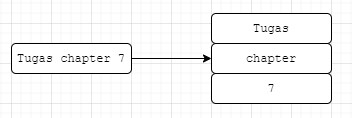
\includegraphics[width=1\textwidth]{figures/1174057/chapter1/1.png}
		\caption{Instalasi Scikit Learn}
		\label{print}
		\end{figure}

		\item Setelah selesai instalasi, pilih salah satu example dari website Scikit. 
		\begin{figure}[H]
		\centering
		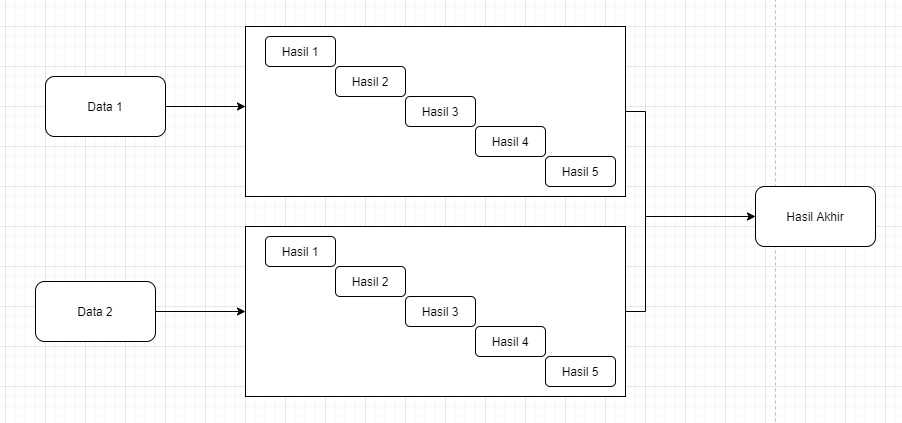
\includegraphics[width=1\textwidth]{figures/1174057/chapter1/2.png}
		\caption{Example}
		\label{print}
		\end{figure}

		\lstinputlisting[firstline=1, lastline=19]{src/1174057/chapter1/example.py}
		\par kemudian coba jalankan, lihat hasilnya
		\begin{figure}[H]
		\centering
		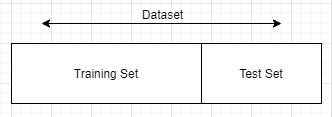
\includegraphics[width=1.5\textwidth]{figures/1174057/chapter1/3.png}
		\caption{Example}
		\label{print}
		\end{figure}

		\item latihan 2 Mencoba Loading an example dataset
		\lstinputlisting[firstline=1, lastline=9]{src/1174057/chapter1/dataset.py}
		\subitem hasil dari data digits
		\begin{figure}[H]
		\centering
		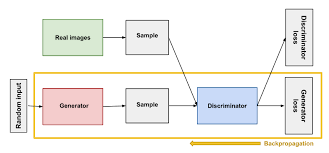
\includegraphics[width=1.5\textwidth]{figures/1174057/chapter1/4.png}
		\caption{Result Data Digits}
		\label{print}
		\end{figure}

		\subitem hasil dari digits.target
		\begin{figure}[H]
		\centering
		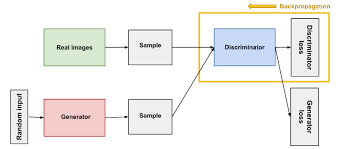
\includegraphics[width=1\textwidth]{figures/1174057/chapter1/5.png}
		\caption{Result digits.target}
		\label{print}
		\end{figure}

		\subitem hasil dari digits.image
		\begin{figure}[H]
		\centering
		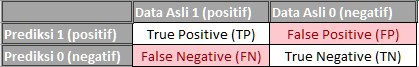
\includegraphics[width=1\textwidth]{figures/1174057/chapter1/6.png}
		\caption{Result digits.image}
		\label{print}
		\end{figure}

		\item latihan 3 Mencoba Learning and predicting
		\lstinputlisting[firstline=1, lastline=9]{src/1174057/chapter1/learning.py}
		\par kemudian coba jalankan, lihat hasilnya
		\begin{figure}[H]
		\centering
		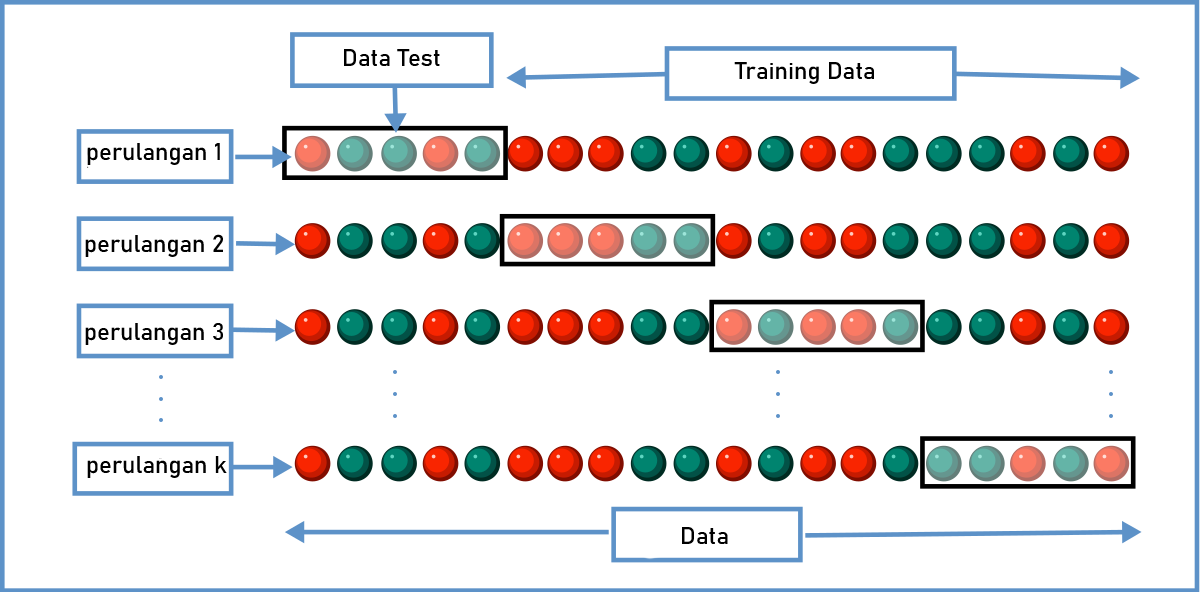
\includegraphics[width=1\textwidth]{figures/1174057/chapter1/7.png}
		\caption{Result Learning and predicting}
		\label{print}
		\end{figure}

		\item latihan 4 Mencoba Model persistence
		\lstinputlisting[firstline=1, lastline=16]{src/1174057/chapter1/modelpersistence.py}
		\par kemudian coba jalankan, lihat hasilnya
		\begin{figure}[H]
		\centering
		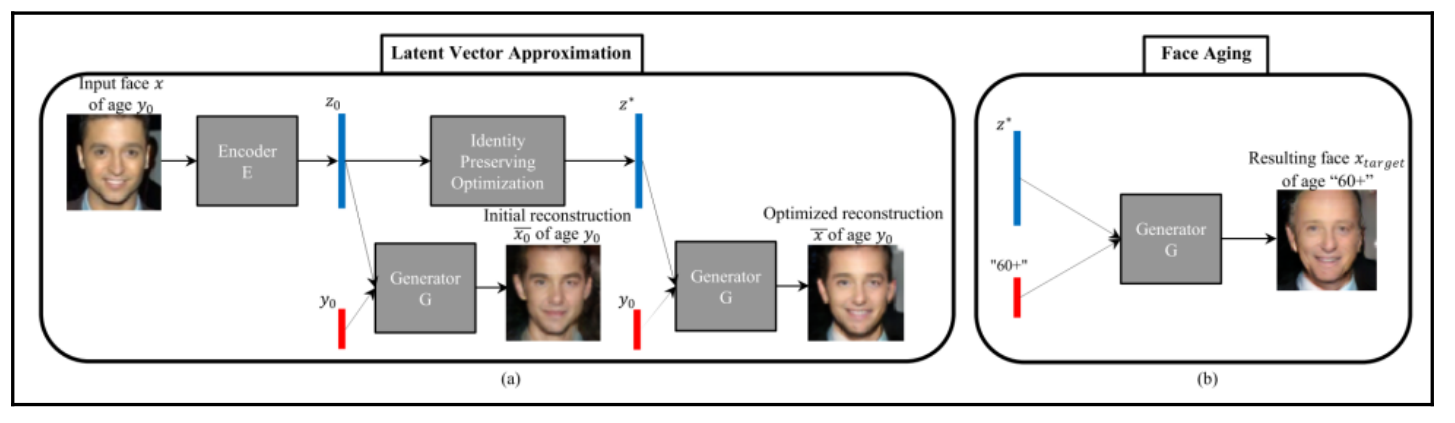
\includegraphics[width=1\textwidth]{figures/1174057/chapter1/8.png}
		\caption{Result Model persistence}
		\label{print}
		\end{figure}

		\item latihan 5 Mencoba Conventions
		\lstinputlisting[firstline=1, lastline=46]{src/1174057/chapter1/modelpersistence.py}
		\par kemudian coba jalankan, lihat hasilnya
		\begin{figure}[H]
		\centering
		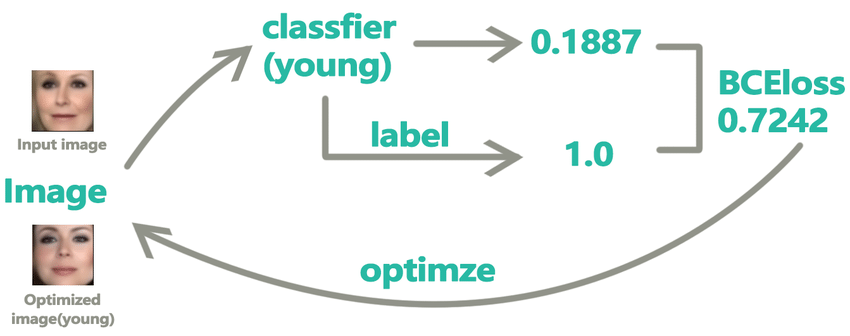
\includegraphics[width=1\textwidth]{figures/1174057/chapter1/9.png}
		\caption{Result Conventions}
		\label{print}
		\end{figure}

	\end{enumerate}

\subsection{Penanganan Error}
	\begin{enumerate}
		\item Screenshoot Error
		\begin{figure}[H]
		\centering
		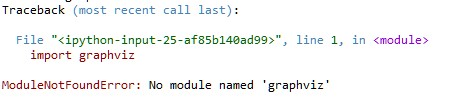
\includegraphics[width=1\textwidth]{figures/1174057/chapter1/error1.png}
		\caption{Error}
		\label{print}
		\end{figure}

		\begin{figure}[H]
		\centering
		\includegraphics[width=1\textwidth]{figures/1174057/chapter1/error2.png}
		\caption{Error}
		\label{print}
		\end{figure}

		\item Tuliskan kode dan jenis error

			\subitem is not defined, xception yang terjadi saat syntax melakukan eksekusi terhadap local name atau global name yang tidak terdefinisi.
			\subitem invalid syntax

		\item Solusi penanganan error

			\subitem Solusinya adalah memastikan variabel atau function yang dipanggil ada atau tidak salah ketik. 
			\subitem Periksa kembali syntax yang dibuat, bisa saja ada kesalahan dalam spasi.
	\end{enumerate}

\subsection{Bukti Tidak Plagiat}
	\begin{figure}[H]
		\centering
		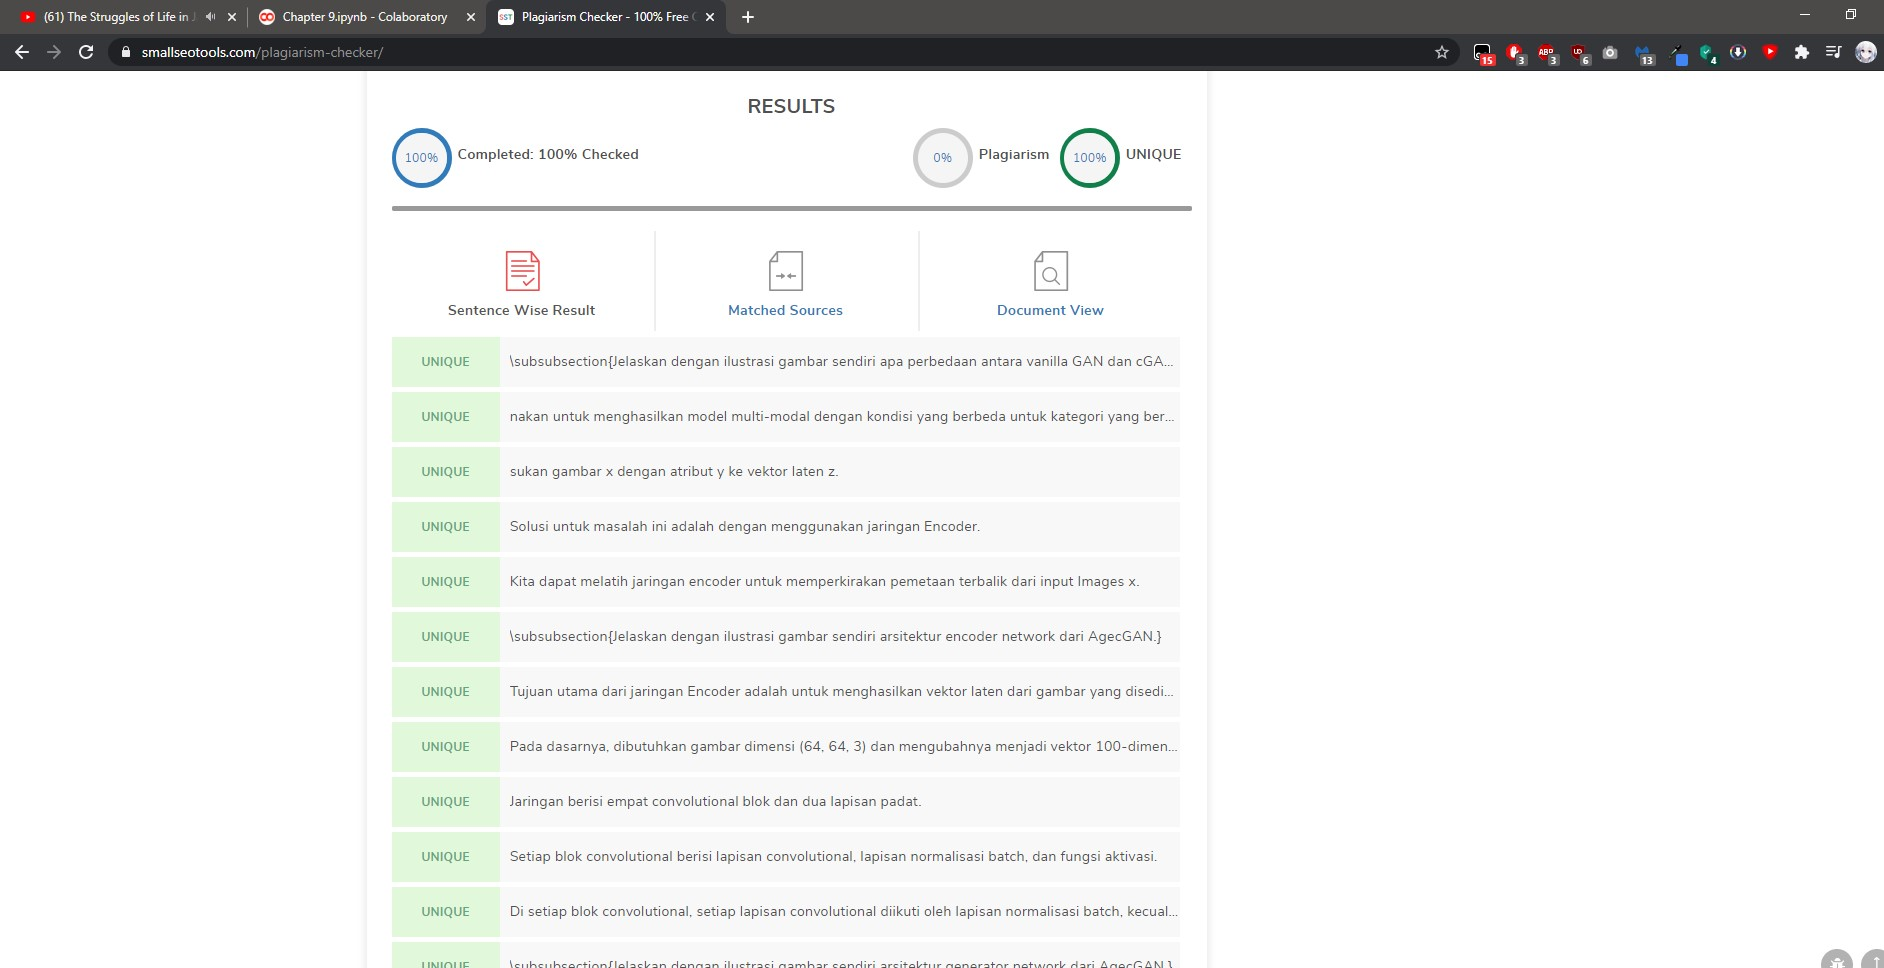
\includegraphics[width=1\textwidth]{figures/1174057/chapter1/plagiat.png}
		\caption{Plagiarisme}
		\label{print}
	\end{figure}
\section{1174034 Ichsan Hizman Hardy}
\subsection{Teori}
\begin{enumerate}
\item Definisi, sejarah, dan perkembangan kecerdasan buatan.
\subitem Kecerdasan buatan (AI) adalah kecerdasan entitas ilmiah. Sistem seperti itu umumnya dianggap sebagai komputer. Kecerdasan diciptakan dan dibangun menjadi mesin (komputer) sehingga dapat berfungsi sebagai manusia. Jenis yang menggunakan kecerdasan buatan, seperti pada bilang sistem pakar, permainan komputer (game), logika fuzzy, jaringan saraf tiruan dan robotika.
\subitem Sejarah kecerdasan buatan dimulai pada pertengahan 1950 di AS. Pada konferensi ilmiah di Dartmouth, M. Minsky, J. McCarthy, A. Newell dan HA Simon adalah yang pertama berbicara tentang 'kecerdasan buatan'. Definisi yang sering dikutip untuk kecerdasan buatan diberikan oleh salah satu pendiri subjek, Marvin Minsky, pada tahun 1966: "Kecerdasan buatan adalah ilmu membuat mesin melakukan hal-hal yang membutuhkan kecerdasan ketika dilakukan oleh manusia." Dengan demikian, ditentukan bahwa kecerdasan buatan adalah ilmu dan bahwa kedua mesin dapat mengambil alih tugas manusia yang membutuhkan kecerdasan manusia.
\par Produk pertama dari kecerdasan buatan adalah pemecah masalah yang umum oleh para peneliti Newell, Shaw dan Simon dari tahun 1960-an. Perangkat ini dapat memecahkan masalah sederhana. Namun, hasil peralatan penelitian tidak dapat digeneralisasi. Pada akhir 1960-an, program lain ditulis dengan ELIZA. Hal ini, Joseph Weizenbaum, seorang peneliti MIT, menyimulasikan sesi terapi.
Pada tahun-tahun berikutnya, sains muda dikembangkan lebih lanjut, yang diproduksi oleh MYCIN pada awal 1970-an dalam sistem inovatif lain berbasis AI. MYCIN dapat membantu dokter mendiagnosis.
Kemajuan dalam sistem kecerdasan buatan didorong oleh kemampuan memori yang terus meningkat dan kinerja prosesor komputer. Sorotan lain adalah superkomputer "Deep Blue" dari IBM, yang dikembangkan pada tahun sembilan puluhan. Sistem ini tidak lagi hanya berdasarkan input manusia, tetapi juga bisa otodidak. Komputer dapat bermain catur pada tahun 1997 dengan juara dunia saat ini. Komputer menang setelah enam pertandingan.
Pada 2016 Raksasa mesin pencari Google menimbulkan kegemparan ketika seorang karyawan melaporkan pada Oktober bahwa Google menggunakan kecerdasan buatan untuk menjawab pertanyaan pencarian. Google menyebut sistem AI-nya 'Brain Rank'. Pada bulan Maret 2016, Google mengumumkan kepada publik bahwa "Peringkat Otak" adalah salah satu dari tiga faktor peringkat paling penting
\item  Definisi supervised learning, klasifikasi, regresi, dan unsupervised learning. Data set, training set dan testing set. 
\subitem Supervised learning adalah jenis pembelajaran di mana kita memiliki variabel input dan variabel output dan menggunakan satu atau lebih algoritma untuk mempelajari fungsi tugas dari input ke output. Tujuannya adalah untuk memperkirakan fungsi penugasan sehingga ketika kita memiliki input baru, kita dapat memprediksi output untuk input ini.
\subitem Klasifikasi adalah salah satu topik utama dalam data mining atau machine learning. Klasifikasi yaitu suatu pengelompokan data dimana data yang digunakan tersebut mempunyai kelas label atau target.
\subitem Regresi adalah Supervised learning tidak hanya mempelajari classifier, tetapi juga mempelajari fungsi yang dapat memprediksi suatu nilai numerik. 
\subitem Data set merupakan sebuah cabang aplikasi dari Artificial Intelligence(AI)/Kecerdasan Buatan yang terfokus kepada pengembangan sebuah sistem yang mampu belajar sendiiri tannpa harus berulang kalai di program oleh manusia(programmer).
\subitem Training set yaitu jika pasangan objek, dan kelas yang menunjuk pada objek tersebut adalah suatu contoh yang telah diberi label akan menghasilkan suatu algoritma pembelajaran.
\subitem Testing set digunakan untuk mengukur sejauh mana classifier berhasil melakukan klasifikasi dengan benar\cite{zhu2009introduction}.
\end{enumerate}

\subsection{Instalasi}
\subsubsection{Instalasi Library Scikit dari Anaconda}
\begin{enumerate}
\item Download aplikasi Anaconda terlebih dahulu. 
\item Install aplikasi Anaconda yang sudah di download tadi. 
\item Simpan aplikasi sesuai folder yang kita pilih lalu next. 
\item Centang Keduanya lalu tekan tombol install. 
\item Setelah itu tunggu sampai proses instalasi selesai lalu jika sudah tekan tombol finish. 
\item Lalu buka command prompt anda dan tuliskan perintah berikut ini untuk mengecek apakah aplikasinya sudah terinstall. 
\item Kemudian ketikkan perinta pip install -U scikit-learn seperti gambar berikut. 
\end{enumerate}
         \begin{figure}[H]
                \includegraphics[width=4cm]{figures/1174034/chapter1/install1.png}
                \centering
                \caption{Instalasi}
            \end{figure}

\subsection{Percobaan}
Mencoba Library
\lstinputlisting[firstline=1, lastline=25]{src/1174034/chapter1/example1.py}
 			\begin{figure}[H]
                \includegraphics[width=4cm]{figures/1174034/chapter1/example1.png}
                \centering
                \caption{Variabel Explore}
            \end{figure}


\subsubsection{Mencoba Loading an example Dataset}
\lstinputlisting[firstline=1, lastline=16]{src/1174034/chapter1/datasett2.py}
		\par kemudian coba jalankan, lihat hasilnya
		\begin{figure}[H]
		\centering
		\includegraphics[width=1.5\textwidth]{figures/1174034/chapter1/dataset1.png}
		\caption{Example}
		\label{print}
		\end{figure}

\subsection{Plagiarism}
\begin{figure}[H]
\centering
\includegraphics[scale=0.5]{figures/1174034/chapter1/plagiat1.png}
\caption{Plagiarism}
\end{figure}

\chapter{Chapter 2}
\input{chapters/chapter2/1174006}

\chapter{Chapter 3}
\input{chapters/chapter3/1174006}

\chapter{Chapter 4}
\input{chapters/chapter4/1174006}

\chapter{Chapter 5}
\input{chapters/chapter5/1174006}

\chapter{Chapter 6}
\input{chapters/chapter6/1174006}

\chapter{Chapter 7}
\input{chapters/chapter7/1174006}

\bibliographystyle{IEEEtran} 
%\def\bibfont{\normalsize}
\bibliography{references}


%%%%%%%%%%%%%%%
%%  The default LaTeX Index
%%  Don't need to add any commands before \begin{document}
\printindex

%%%% Making an index
%% 
%% 1. Make index entries, don't leave any spaces so that they
%% will be sorted correctly.
%% 
%% \index{term}
%% \index{term!subterm}
%% \index{term!subterm!subsubterm}
%% 
%% 2. Run LaTeX several times to produce <filename>.idx
%% 
%% 3. On command line, type  makeindx <filename> which
%% will produce <filename>.ind 
%% 
%% 4. Type \printindex to make the index appear in your book.
%% 
%% 5. If you would like to edit <filename>.ind 
%% you may do so. See docs.pdf for more information.
%% 
%%%%%%%%%%%%%%%%%%%%%%%%%%%%%%

%%%%%%%%%%%%%% Making Multiple Indices %%%%%%%%%%%%%%%%
%% 1. 
%% \usepackage{multind}
%% \makeindex{book}
%% \makeindex{authors}
%% \begin{document}
%% 
%% 2.
%% % add index terms to your book, ie,
%% \index{book}{A term to go to the topic index}
%% \index{authors}{Put this author in the author index}
%% 
%% \index{book}{Cows}
%% \index{book}{Cows!Jersey}
%% \index{book}{Cows!Jersey!Brown}
%% 
%% \index{author}{Douglas Adams}
%% \index{author}{Boethius}
%% \index{author}{Mark Twain}
%% 
%% 3. On command line type 
%% makeindex topic 
%% makeindex authors
%% 
%% 4.
%% this is a Wiley command to make the indices print:
%% \multiprintindex{book}{Topic index}
%% \multiprintindex{authors}{Author index}

\end{document}

